%%%%%%%%%%%%%%%%%%%%%%%%%%%%%%%%%%%%
% Slide options
%%%%%%%%%%%%%%%%%%%%%%%%%%%%%%%%%%%%

% Option 1: Slides with solutions

\documentclass[slidestop,compress,mathserif]{beamer}
\newcommand{\soln}[1]{\textit{#1}}
\newcommand{\solnGr}[1]{#1}

% Option 2: Handouts without solutions

%\documentclass[11pt,containsverbatim,handout]{beamer}
%\usepackage{pgfpages}
%\pgfpagesuselayout{4 on 1}[letterpaper,landscape,border shrink=5mm]
%\newcommand{\soln}[1]{ }
%\newcommand{\solnGr}{ }


%%%%%%%%%%%%%%%%%%%%%%%%%%%%%%%%%%%%
% Style
%%%%%%%%%%%%%%%%%%%%%%%%%%%%%%%%%%%%

\def\chp3@path{../../Chp 3}
\input{../../lec_style.tex}


%%%%%%%%%%%%%%%%%%%%%%%%%%%%%%%%%%%%
% Preamble
%%%%%%%%%%%%%%%%%%%%%%%%%%%%%%%%%%%%

\title[Lecture 9]{MA213: Lecture 9}
\subtitle{Module 2: Probability, Random Variables, and Distributions}
\author{OpenIntro Statistics, 4th Edition}
\institute{$\:$ \\ {\footnotesize Based on slides developed by Mine \c{C}etinkaya-Rundel of OpenIntro. \\
The slides may be copied, edited, and/or shared via the \webLink{http://creativecommons.org/licenses/by-sa/3.0/us/}{CC BY-SA license.} \\
Some images may be included under fair use guidelines (educational purposes).}}
\date{}

%%%%%%%%%%%%%%%%%%%%%%%%%%%%%%%%%%%%
% Begin document
%%%%%%%%%%%%%%%%%%%%%%%%%%%%%%%%%%%%

\begin{document}


%%%%%%%%%%%%%%%%%%%%%%%%%%%%%%%%%%%%
% Title page
%%%%%%%%%%%%%%%%%%%%%%%%%%%%%%%%%%%%

{
\addtocounter{framenumber}{-1} 
{\removepagenumbers 
\usebackgroundtemplate{\includegraphics[width=\paperwidth]{../../OpenIntro_Grid_4_3-01.jpg}}
\begin{frame}

\hfill \includegraphics[width=20mm]{../../oiLogo_highres}

\titlepage

\end{frame}
}
}


%%%%%%%%%%%%%%%%%%%%%%%%%%%%%%%%%%%%
% Recap/Agenda 
%%%%%%%%%%%%%%%%%%%%%%%%%%%%%%%%%%%%
% TODO better formatting
\begin{frame}
    \frametitle{Module 2: Probability, Random Variables, and Distributions}
    \begin{itemize}
        \item \hl{Previously: } Random Variables (Chapter 3.4)
        \item \hl{This time: } Continuous Distributions (Chapter 3.5)
        \item \hl{Reading: } Chapter 4.1 for next time
        \item \hl{Deadlines/Announcements: } Quiz 1 in discussions this week, HW 2.1 due today
    \end{itemize}
    
\end{frame}
    

%%%%%%%%%%%%%%%%%%%%%%%%%%%%%%%%%%%%
% Sections
%%%%%%%%%%%%%%%%%%%%%%%%%%%%%%%%%%%%

%%%%%%%%%%%%%%%%%%%%%%%%%%%%%%%%%%%%

\section{Continuous distributions}

%%%%%%%%%%%%%%%%%%%%%%%%%%%%%%%%%%%%

\begin{frame}
\frametitle{Continuous distributions}

\begin{itemize}

\item Below is a histogram of the distribution of heights of US adults. 

\item The proportion of data that falls in the shaded bins gives the probability that a randomly sampled US adult is between 180 cm and 185 cm (about 5'11" to 6'1").

\end{itemize}

\begin{center}
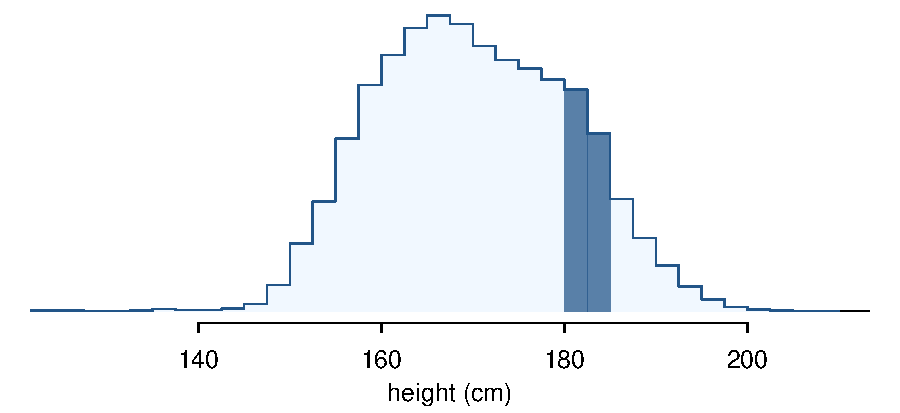
\includegraphics[width=\textwidth]{\chp3@path/3-5_continuous_distributions/figures/usHeightsHist180185/usHeightsHist180185}
\end{center}


\end{frame}

%%%%%%%%%%%%%%%%%%%%%%%%%%%%%%%%%%%%

\subsection{From histograms to continuous distributions}

\begin{frame}
\frametitle{From histograms to continuous distributions}

Since height is a continuous numerical variable, its \hl{probability density function} is a smooth curve.

\begin{center}
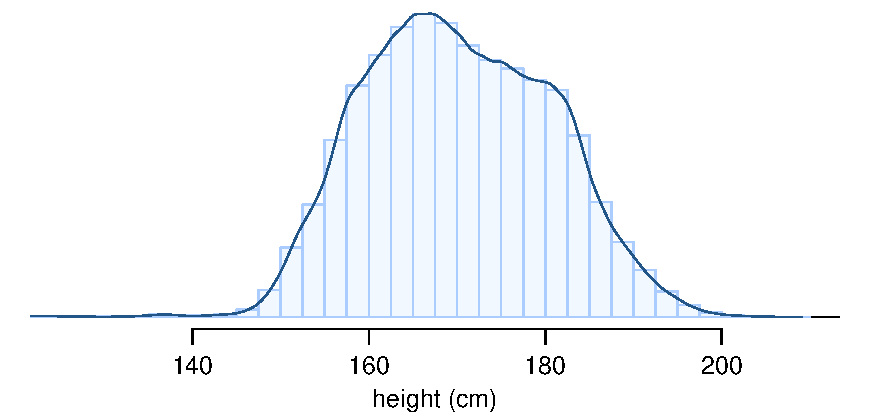
\includegraphics[width=\textwidth]{\chp3@path/3-5_continuous_distributions/figures/fdicHeightContDist/fdicHeightContDist}
\end{center}

\end{frame}

%%%%%%%%%%%%%%%%%%%%%%%%%%%%%%%%%%%%

\subsection{Probabilities from continuous distributions}

\begin{frame}
\frametitle{Probabilities from continuous distributions}

Therefore, the probability that a randomly sampled US adult is between 180 cm and 185 cm can also be estimated as the shaded area under the curve.

\begin{center}
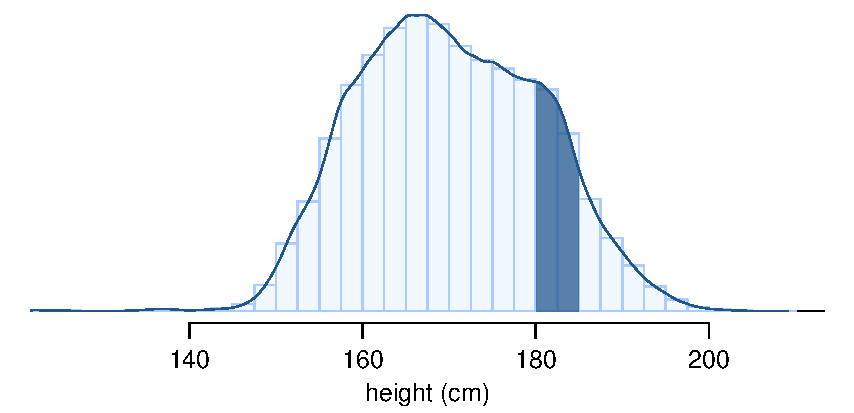
\includegraphics[width=\textwidth]{\chp3@path/3-5_continuous_distributions/figures/fdicHeightContDistFilled/fdicHeightContDistFilled}
\end{center}


\end{frame}

%%%%%%%%%%%%%%%%%%%%%%%%%%%%%%%%%%%%

\begin{frame}
\frametitle{By definition...}

Since continuous probabilities are estimated as ``the area under the curve", the probability of a person being exactly 180 cm (or any exact value) is defined as 0.

\begin{center}
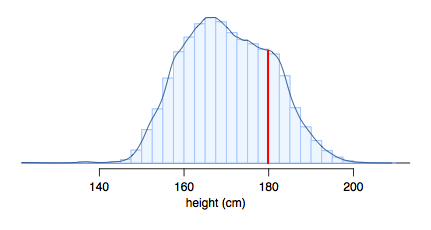
\includegraphics[width=0.8\textwidth]{\chp3@path/3-5_continuous_distributions/figures/fdicHeightContDist180}
\end{center}

\end{frame}

%%%%%%%%%%%%%%%%%%%%%%%%%%%%%%%%%%%%

\section{R Demonstration}

%%%%%%%%%%%%%%%%%%%%%%%%%%%%%%%%%%%%

\section{Edfinity quiz}

%%%%%%%%%%%%%%%%%%%%%%%%%%%%%%%%%%%%

%%%%%%%%%%%%%%%%%%%%%%%%%%%%%%%%%%%%
% End document
%%%%%%%%%%%%%%%%%%%%%%%%%%%%%%%%%%%%

\end{document}